\section{Composer\-View Class Reference}
\label{classComposerView}\index{ComposerView@{ComposerView}}
Main view.  


{\tt \#include $<$composerview.h$>$}

Inheritance diagram for Composer\-View::\begin{figure}[H]
\begin{center}
\leavevmode
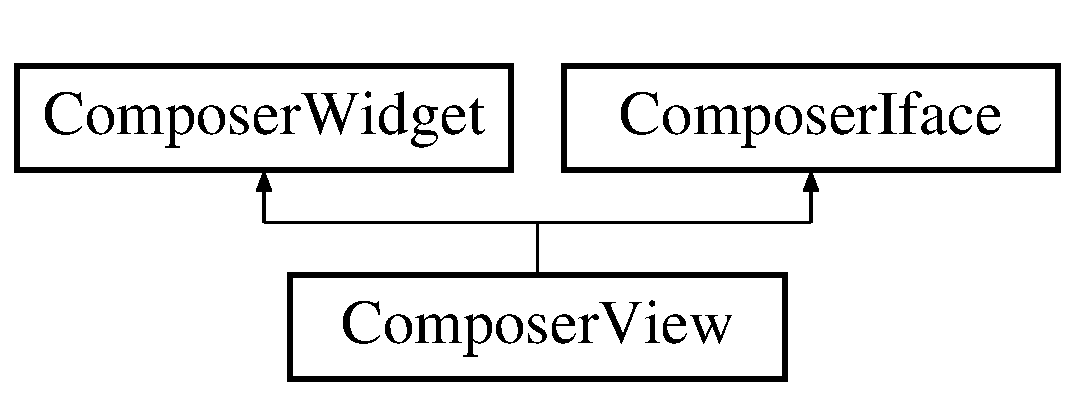
\includegraphics[height=2cm]{classComposerView}
\end{center}
\end{figure}
\subsection*{Public Slots}
\begin{CompactItemize}
\item 
void {\bf open\-URL} (const KURL \&url)
\item 
void {\bf open\-URL} (QString url)
\item 
void {\bf print} (QPainter $\ast$, int height, int width)
\item 
void {\bf t\_\-type\_\-changed} (int)
\item 
QWidget $\ast$ {\bf w\_\-show} (QWidget $\ast$, QWidget $\ast$)
\end{CompactItemize}
\subsection*{Signals}
\begin{CompactItemize}
\item 
void {\bf signal\-Change\-Caption} (const QString \&text)
\item 
void {\bf signal\-Change\-Statusbar} (const QString \&text)
\end{CompactItemize}
\subsection*{Public Member Functions}
\begin{CompactItemize}
\item 
{\bf Composer\-View} (QWidget $\ast$parent)
\item 
QString {\bf current\-URL} ()
\item 
virtual {\bf $\sim$Composer\-View} ()
\end{CompactItemize}
\subsection*{Public Attributes}
\begin{CompactItemize}
\item 
QWidget $\ast$ {\bf d}
\item 
QWidget $\ast$ {\bf r}
\item 
{\bf Transistor} $\ast$ {\bf t}
\item 
QWidget $\ast$ {\bf w}
\end{CompactItemize}
\subsection*{Private Slots}
\begin{CompactItemize}
\item 
void {\bf character\_\-chosen} (int)
\item 
void {\bf resize\-Event} (QResize\-Event $\ast$)
\item 
void {\bf slot\-On\-URL} (const QString \&url)
\item 
void {\bf slot\-Set\-Title} (const QString \&title)
\end{CompactItemize}
\subsection*{Private Attributes}
\begin{CompactItemize}
\item 
KParts::Read\-Only\-Part $\ast$ {\bf m\_\-html}
\end{CompactItemize}


\subsection{Detailed Description}
Main view. 

\begin{Desc}
\item[Author:]sebastian $<${\tt sebastian.bw@freenet.de}$>$ \end{Desc}
\begin{Desc}
\item[Version:]0.1 \end{Desc}




\subsection{Constructor \& Destructor Documentation}
\index{ComposerView@{Composer\-View}!ComposerView@{ComposerView}}
\index{ComposerView@{ComposerView}!ComposerView@{Composer\-View}}
\subsubsection{\setlength{\rightskip}{0pt plus 5cm}Composer\-View::Composer\-View (QWidget $\ast$ {\em parent})}\label{classComposerView_d059e3c900af7e133d6804584f95316a}


\index{ComposerView@{Composer\-View}!~ComposerView@{$\sim$ComposerView}}
\index{~ComposerView@{$\sim$ComposerView}!ComposerView@{Composer\-View}}
\subsubsection{\setlength{\rightskip}{0pt plus 5cm}Composer\-View::$\sim$Composer\-View ()\hspace{0.3cm}{\tt  [virtual]}}\label{classComposerView_207b51aebba5131f90aa903795c98772}




\subsection{Member Function Documentation}
\index{ComposerView@{Composer\-View}!character_chosen@{character\_\-chosen}}
\index{character_chosen@{character\_\-chosen}!ComposerView@{Composer\-View}}
\subsubsection{\setlength{\rightskip}{0pt plus 5cm}void Composer\-View::character\_\-chosen (int)\hspace{0.3cm}{\tt  [private, virtual, slot]}}\label{classComposerView_c9c3e0c0edd13829d6dd945b8a46bbe1}




Reimplemented from {\bf Composer\-Widget} {\rm (p.\,\pageref{classComposerWidget_c9c3e0c0edd13829d6dd945b8a46bbe1})}.\index{ComposerView@{Composer\-View}!currentURL@{currentURL}}
\index{currentURL@{currentURL}!ComposerView@{Composer\-View}}
\subsubsection{\setlength{\rightskip}{0pt plus 5cm}QString Composer\-View::current\-URL ()}\label{classComposerView_2a810dff322ac5b0ccfdd666b79c9443}


\index{ComposerView@{Composer\-View}!openURL@{openURL}}
\index{openURL@{openURL}!ComposerView@{Composer\-View}}
\subsubsection{\setlength{\rightskip}{0pt plus 5cm}void Composer\-View::open\-URL (const KURL \& {\em url})\hspace{0.3cm}{\tt  [slot]}}\label{classComposerView_bd29ea8da04eb211ed2f5617c6ce1efb}


\index{ComposerView@{Composer\-View}!openURL@{openURL}}
\index{openURL@{openURL}!ComposerView@{Composer\-View}}
\subsubsection{\setlength{\rightskip}{0pt plus 5cm}void Composer\-View::open\-URL (QString {\em url})\hspace{0.3cm}{\tt  [virtual, slot]}}\label{classComposerView_1d669cfc5a2d59fafee1b0c99df3a957}




Implements {\bf Composer\-Iface} {\rm (p.\,\pageref{classComposerIface_3deb991ea51d92a58332714d156f1389})}.\index{ComposerView@{Composer\-View}!print@{print}}
\index{print@{print}!ComposerView@{Composer\-View}}
\subsubsection{\setlength{\rightskip}{0pt plus 5cm}void Composer\-View::print (QPainter $\ast$, int {\em height}, int {\em width})\hspace{0.3cm}{\tt  [slot]}}\label{classComposerView_049cd1d13f85a362dcd3c318f3b4c5b0}


\index{ComposerView@{Composer\-View}!resizeEvent@{resizeEvent}}
\index{resizeEvent@{resizeEvent}!ComposerView@{Composer\-View}}
\subsubsection{\setlength{\rightskip}{0pt plus 5cm}void Composer\-View::resize\-Event (QResize\-Event $\ast$)\hspace{0.3cm}{\tt  [private, slot]}}\label{classComposerView_566d9b8eed7e434eda4a730423f8416c}


\index{ComposerView@{Composer\-View}!signalChangeCaption@{signalChangeCaption}}
\index{signalChangeCaption@{signalChangeCaption}!ComposerView@{Composer\-View}}
\subsubsection{\setlength{\rightskip}{0pt plus 5cm}void Composer\-View::signal\-Change\-Caption (const QString \& {\em text})\hspace{0.3cm}{\tt  [signal]}}\label{classComposerView_1640e1a8403c83b28da4a8c144e72a24}


\index{ComposerView@{Composer\-View}!signalChangeStatusbar@{signalChangeStatusbar}}
\index{signalChangeStatusbar@{signalChangeStatusbar}!ComposerView@{Composer\-View}}
\subsubsection{\setlength{\rightskip}{0pt plus 5cm}void Composer\-View::signal\-Change\-Statusbar (const QString \& {\em text})\hspace{0.3cm}{\tt  [signal]}}\label{classComposerView_a483002718991e728fbec2ad1de19bec}


\index{ComposerView@{Composer\-View}!slotOnURL@{slotOnURL}}
\index{slotOnURL@{slotOnURL}!ComposerView@{Composer\-View}}
\subsubsection{\setlength{\rightskip}{0pt plus 5cm}void Composer\-View::slot\-On\-URL (const QString \& {\em url})\hspace{0.3cm}{\tt  [private, slot]}}\label{classComposerView_503a57aeabd28ebad3fcdffb7dd30bcf}


\index{ComposerView@{Composer\-View}!slotSetTitle@{slotSetTitle}}
\index{slotSetTitle@{slotSetTitle}!ComposerView@{Composer\-View}}
\subsubsection{\setlength{\rightskip}{0pt plus 5cm}void Composer\-View::slot\-Set\-Title (const QString \& {\em title})\hspace{0.3cm}{\tt  [private, slot]}}\label{classComposerView_8ec7516cd95ae475094889b9a2ec4341}


\index{ComposerView@{Composer\-View}!t_type_changed@{t\_\-type\_\-changed}}
\index{t_type_changed@{t\_\-type\_\-changed}!ComposerView@{Composer\-View}}
\subsubsection{\setlength{\rightskip}{0pt plus 5cm}void Composer\-View::t\_\-type\_\-changed (int)\hspace{0.3cm}{\tt  [slot]}}\label{classComposerView_5c482ee5ba4ea523a76dbc40fa91456e}


\index{ComposerView@{Composer\-View}!w_show@{w\_\-show}}
\index{w_show@{w\_\-show}!ComposerView@{Composer\-View}}
\subsubsection{\setlength{\rightskip}{0pt plus 5cm}QWidget $\ast$ Composer\-View::w\_\-show (QWidget $\ast$, QWidget $\ast$)\hspace{0.3cm}{\tt  [slot]}}\label{classComposerView_d0d650902f9540d47a9dd405f6baed22}




\subsection{Member Data Documentation}
\index{ComposerView@{Composer\-View}!d@{d}}
\index{d@{d}!ComposerView@{Composer\-View}}
\subsubsection{\setlength{\rightskip}{0pt plus 5cm}QWidget $\ast$ {\bf Composer\-View::d}}\label{classComposerView_8277e0910d750195b448797616e091ad}


\index{ComposerView@{Composer\-View}!m_html@{m\_\-html}}
\index{m_html@{m\_\-html}!ComposerView@{Composer\-View}}
\subsubsection{\setlength{\rightskip}{0pt plus 5cm}KParts::Read\-Only\-Part$\ast$ {\bf Composer\-View::m\_\-html}\hspace{0.3cm}{\tt  [private]}}\label{classComposerView_73aa6a5809b4d9db65099c4f54c9e4c8}


\index{ComposerView@{Composer\-View}!r@{r}}
\index{r@{r}!ComposerView@{Composer\-View}}
\subsubsection{\setlength{\rightskip}{0pt plus 5cm}QWidget $\ast$ {\bf Composer\-View::r}}\label{classComposerView_4b43b0aee35624cd95b910189b3dc231}


\index{ComposerView@{Composer\-View}!t@{t}}
\index{t@{t}!ComposerView@{Composer\-View}}
\subsubsection{\setlength{\rightskip}{0pt plus 5cm}{\bf Transistor}$\ast$ {\bf Composer\-View::t}}\label{classComposerView_e358efa489f58062f10dd7316b65649e}


\index{ComposerView@{Composer\-View}!w@{w}}
\index{w@{w}!ComposerView@{Composer\-View}}
\subsubsection{\setlength{\rightskip}{0pt plus 5cm}QWidget$\ast$ {\bf Composer\-View::w}}\label{classComposerView_f1290186a5d0b1ceab27f4e77c0c5d68}




The documentation for this class was generated from the following files:\begin{CompactItemize}
\item 
/home/bastl/Kdevel/keda/composer/{\bf composerview.h}\item 
/home/bastl/Kdevel/keda/composer/{\bf composerview.cpp}\item 
/home/bastl/Kdevel/keda/composer/{\bf composerview.moc}\end{CompactItemize}
